\chapter{Evaluation}

\section{Customer Requirements}

These are the original objectives specified by the client at the analysis stage of making this system.

\textbf{General Objectives}

\begin{itemize}
	\item To have an interactive and easily navigable graphical user interface, applying a suitable colour scheme and layout
	\item To make the database concise and adjustable
	\item To create various lessons, with a wide range of challenges, which effectively teach students how to do trigonometry and Pythagoras
	\item To create tasks which are relevant to the lessons to be completed by the user in order to test their progress
	\item To allow this progress to be recorded in an easily accessible and readable database
	\item To incorporate algorithms which find and/or check the solution given by the user accurately and give clear and easy to read outputs to correspond with said inputs
	\item To have some access restrictions to certain levels of user
	\item To make the program accessible only from various computers with permissions
\end{itemize}

\textbf{Specific Objectives}

\begin{itemize}
	\item To create a teaching program that uses the new GCSE Maths curriculum, as lots of resources will soon be out of date
	\item To include the following topics: Trigonometry, Pythagoras, 3D Trigonometry, 3D Pythagoras
	\item To include a range of difficulty levels, which can challenge every user's level of ability
	\item Use drag and drop, text boxes and drop down menus for inputs
	\item To include interactive 2D graphics which give a clearer idea of the method being shown to the user
	\item To have a database which can be accessed by different computers online
	\item Use a specific, continuous and attractive colour scheme in every window
	\item To have medium sized, highly visible icons
	\item To have all input buttons randomised to avoid double clicking and guessing from memory
	\item To have small error message windows which pop up and disappear on a timer
	\item To include images and shapes which contrast the colour scheme so they are visible and readable
\end{itemize}

\textbf{Core Objectives}

\begin{itemize}
	\item To create a teaching program that uses the new GCSE Maths curriculum, as lots of resources will soon be out of date
	\item To make the database easy to access and easy to read
	\item To include primarily trigonometry based topics, such as how to use the sine, cosine and tan rules
	\item To include an initial, moderate difficulty in order to cater for a majority of students
	\item To make the database functional and able to store the requested details
\end{itemize}

\textbf{Other Objectives}

\begin{itemize}
	\item To position buttons, text boxes and drag and drop boxes in within the layout of the graphical user interface in such a way that cheating and lucky guessing can be minimised
	\item To make the database adjustable if necessary
	\item Use a more interesting range of input types like drawing boxes rather than just clicking and typing
	\item To include a wider range of difficulties to challenge every student on the right level for them
	\item To include a wider range of topics such as pythagoras, then 3D trigonometry and 3D pythagoras
\end{itemize}

\subsection{Objective: }

To have an interactive and easily navigable graphical user interface, applying a suitable colour scheme and layout

\subsubsection{Objective Met?}

Yes/no 

\subsubsection{Evidence: }

Evidence

\subsection{Objective: }

To make the database concise and adjustable

\subsubsection{Objective Met?}

Yes/no 

\subsubsection{Evidence: }

Evidence

\subsection{Objective: }

To create various lessons, with a wide range of challenges, which effectively teach students how to do trigonometry and Pythagoras

\subsubsection{Objective Met?}

Yes/no 

\subsubsection{Evidence: }

Evidence

\subsection{Objective: }

To create tasks which are relevant to the lessons to be completed by the user in order to test their progress

\subsubsection{Objective Met?}

Yes/no 

\subsubsection{Evidence: }

Evidence

\subsection{Objective: }

To allow this progress to be recorded in an easily accessible and readable database

\subsubsection{Objective Met?}

Yes/no 

\subsubsection{Evidence: }

Evidence

\subsection{Objective: }

To incorporate algorithms which find and/or check the solution given by the user accurately and give clear and easy to read outputs to correspond with said inputs

\subsubsection{Objective Met?}

Yes/no 

\subsubsection{Evidence: }

Evidence

\subsection{Objective: }

To have some access restrictions to certain levels of user

\subsubsection{Objective Met?}

Yes/no 

\subsubsection{Evidence: }

Evidence

\subsection{Objective: }

To make the program accessible only from various computers with permissions

\subsubsection{Objective Met?}

Yes/no 

\subsubsection{Evidence: }

Evidence

\subsection{Objective: }

To create a teaching program that uses the new GCSE Maths curriculum, as lots of resources will soon be out of date

\subsubsection{Objective Met?}

Yes/no 

\subsubsection{Evidence: }

Evidence

\subsection{Objective: }

To include the following topics: Trigonometry, Pythagoras, 3D Trigonometry, 3D Pythagoras

\subsubsection{Objective Met?}

Yes/no 

\subsubsection{Evidence: }

Evidence

\subsection{Objective: }

To include a range of difficulty levels, which can challenge every user's level of ability

\subsubsection{Objective Met?}

Yes/no 

\subsubsection{Evidence: }

Evidence

\subsection{Objective: }

Use drag and drop, text boxes and drop down menus for inputs

\subsubsection{Objective Met?}

Yes/no 

\subsubsection{Evidence: }

Evidence

\subsection{Objective: }

To include interactive 2D graphics which give a clearer idea of the method being shown to the user

\subsubsection{Objective Met?}

Yes/no 

\subsubsection{Evidence: }

Evidence

\subsection{Objective: }

To have a database which can be accessed by different computers online

\subsubsection{Objective Met?}

Yes/no 

\subsubsection{Evidence: }

Evidence

\subsection{Objective: }

Use a specific, continuous and attractive colour scheme in every window

\subsubsection{Objective Met?}

Yes/no 

\subsubsection{Evidence: }

Evidence

\subsection{Objective: }

To have medium sized, highly visible icons

\subsubsection{Objective Met?}

Yes/no 

\subsubsection{Evidence: }

Evidence

\subsection{Objective: }

To have all input buttons randomised to avoid double clicking and guessing from memory

\subsubsection{Objective Met?}

Yes/no 

\subsubsection{Evidence: }

Evidence

\subsection{Objective: }

To have small error message windows which pop up and disappear on a timer

\subsubsection{Objective Met?}

Yes/no 

\subsubsection{Evidence: }

Evidence

\subsection{Objective: }

To include images and shapes which contrast the colour scheme so they are visible and readable

\subsubsection{Objective Met?}

Yes/no 

\subsubsection{Evidence: }

Evidence

\subsection{Objective: }

To create a teaching program that uses the new GCSE Maths curriculum, as lots of resources will soon be out of date

\subsubsection{Objective Met?}

Yes/no 

\subsubsection{Evidence: }

Evidence

\subsection{Objective: }

To make the database easy to access and easy to read

\subsubsection{Objective Met?}

Yes/no 

\subsubsection{Evidence: }

Evidence

\subsection{Objective: }

To include primarily trigonometry based topics, such as how to use the sine, cosine and tan rules

\subsubsection{Objective Met?}

Yes/no 

\subsubsection{Evidence: }

Evidence

\subsection{Objective: }

To include an initial, moderate difficulty in order to cater for a majority of students

\subsubsection{Objective Met?}

Yes/no 

\subsubsection{Evidence: }

Evidence

\subsection{Objective: }

To make the database functional and able to store the requested details

\subsubsection{Objective Met?}

Yes/no 

\subsubsection{Evidence: }

Evidence

\subsection{Objective: }

To position buttons, text boxes and drag and drop boxes in within the layout of the graphical user interface in such a way that cheating and lucky guessing can be minimised

\subsubsection{Objective Met?}

Yes/no 

\subsubsection{Evidence: }

Evidence

\subsection{Objective: }

To make the database adjustable if necessary

\subsubsection{Objective Met?}

Yes/no 

\subsubsection{Evidence: }

Evidence

\subsection{Objective: }

Use a more interesting range of input types like drawing boxes rather than just clicking and typing

\subsubsection{Objective Met?}

Yes/no 

\subsubsection{Evidence: }

Evidence

\subsection{Objective: }

To include a wider range of difficulties to challenge every student on the right level for them

\subsubsection{Objective Met?}

Yes/no 

\subsubsection{Evidence: }

Evidence

\subsection{Objective: }

To include a wider range of topics such as pythagoras, then 3D trigonometry and 3D pythagoras

\subsubsection{Objective Met?}

Yes/no 

\subsubsection{Evidence: }

Evidence
















 
\section{Effectiveness}

%include as many subsections as necessary for your objectives
\subsection{Objective Evaluation}






\section{Learnability}

When I first consulted my client I took into account how much experience they have already had using software such as my system. They are comfortable using the internet, so with the assistance of the user manual they should have no problem installing Python 3.4 and PyQt4. They, along with the other people the client intends to use this system with, have all had experience using similar educational maths programs, such as MyMaths, which have essentially the same purpose as my system. Therefore I tried to make some aspects of the system somewhat similar to the ones conventionally used in educational maths programs, such as the layout, including the navigation of the system, the topics, and the rules of saving and popping error messages, such as making sure all questions have been attempted. None the less, this system would probably be easy enough for less experienced users anyway, as generally the buttons are clearly labelled, appropriately sized, and organised in a convenient way (branch menu). Although some users may have issues finding the exact right topic in the sub-menus, being a reason for the big red return buttons which make it easy to go back and try another menu.

\begin{figure}[H]
	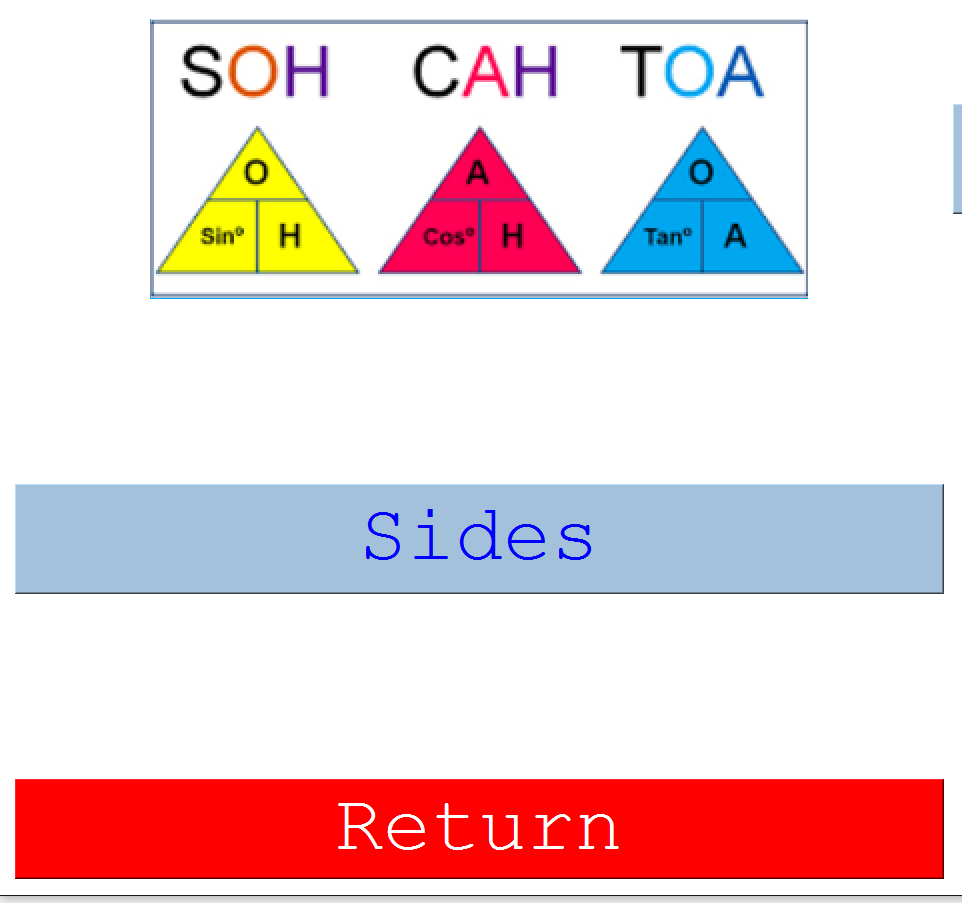
\includegraphics{C:/Users/Jordan/git/COMP4Coursework2/Evaluation/learnability_1}
	\caption{An example of the return buttons used to make navigating the sub-menus easier}
\end{figure}

When designing the system I kept in mind the fact that saving data can be a more complex function if it is done manually, especially by an inexperienced user, so I made all of the database functions automatic; they occur when the user simply clicks a button to finish a homework, or opens the progress screen. This cancels out the need for users to learn new skills which they might not have already learned from using similar systems.

\begin{figure}[H]
	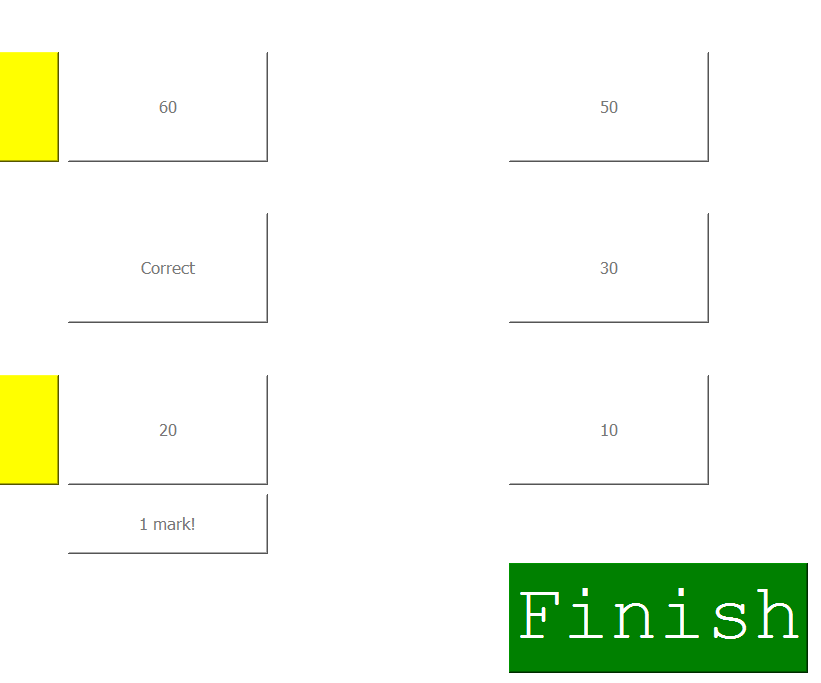
\includegraphics{C:/Users/Jordan/git/COMP4Coursework2/Evaluation/learnability_2}
	\caption{The finish button being clicked to automatically save progress for the user}
\end{figure}

\begin{figure}[H]
	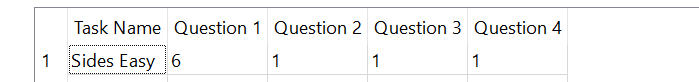
\includegraphics{C:/Users/Jordan/git/COMP4Coursework2/Evaluation/learnability_3}
	\caption{The record which was just saved immediately being updated to the database}
\end{figure}

I also endeavoured to make the database itself very easy to access and understand internally in the system; the system accesses the information from a separate file and displays it in a window in the program, which can be accessed by the user very quickly from the home screen, and even queried for specific details should the user be searching for a specific record. the options in hte combo boxes are as clear as I can make them to make it easier for the user to determine how to use the query function when they try it for the first time.

\begin{figure}[H]
	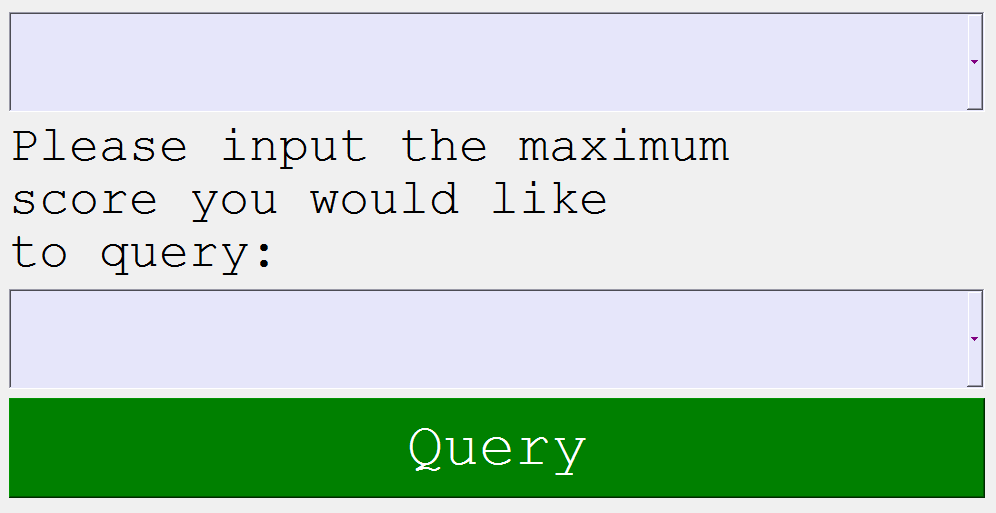
\includegraphics{C:/Users/Jordan/git/COMP4Coursework2/Evaluation/learnability_4}
	\caption{An example of the database being queried for easy access to specific records}
\end{figure}

Error messages were also incorporated to help the user understand why the sytem isn't working as they expected, should they fail to answer a question properly and try to proceed to the next page and be unsure why they cannot.

\begin{figure}[H]
	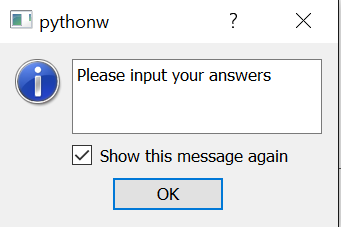
\includegraphics{C:/Users/Jordan/git/COMP4Coursework2/Evaluation/learnability_5}
	\caption{An example of an error message telling the user why they cannot proceed}
\end{figure}

Generally, this system is very easy to use, even for people with little experience with such software, and care has been taken to ensure that the interface is very clear and the error messages are sufficient to help a user fix a progression related problem should they need the help. The only concern is that the user has no way to reset the database internally, so once they start using the system they have to either keep their progress or delete the database file manually.

\section{Usability}

\section{Maintainability}

\section{Suggestions for Improvement}



















\section{End User Evidence}

The following images are from a feedback form which I provided to the client so they could convey to me the extent to which they were satisfied with the system.

\begin{figure}[H]
	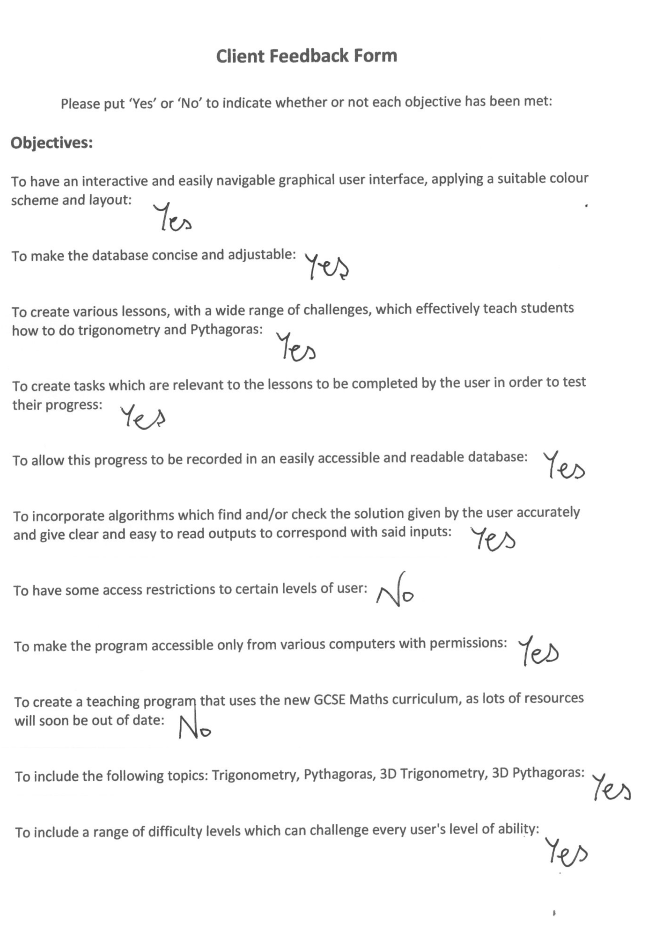
\includegraphics{C:/Users/Jordan/git/COMP4Coursework2/Evaluation/client_feedback_1}
\end{figure}

\begin{figure}[H]
	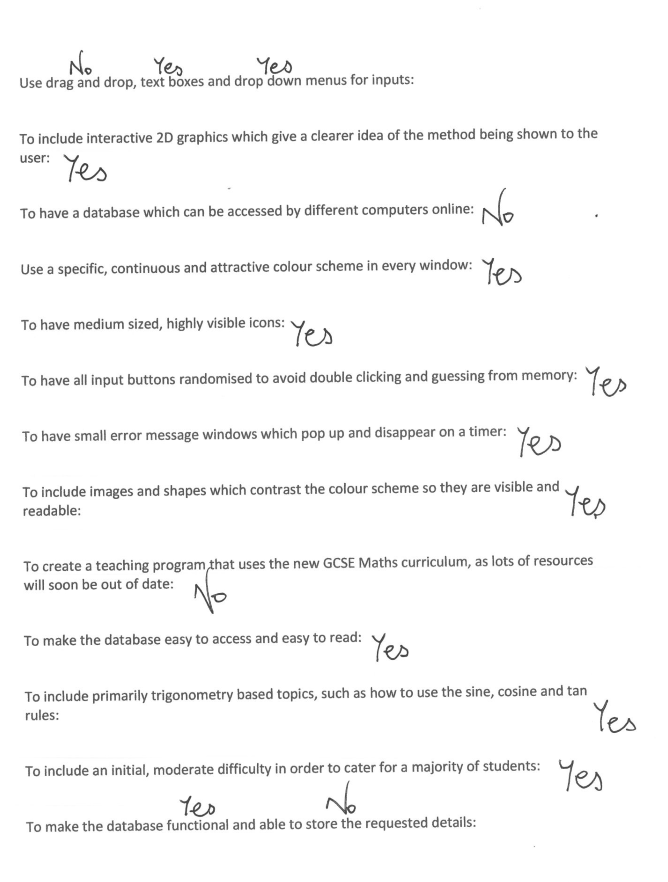
\includegraphics{C:/Users/Jordan/git/COMP4Coursework2/Evaluation/client_feedback_2}
\end{figure}

\begin{figure}[H]
	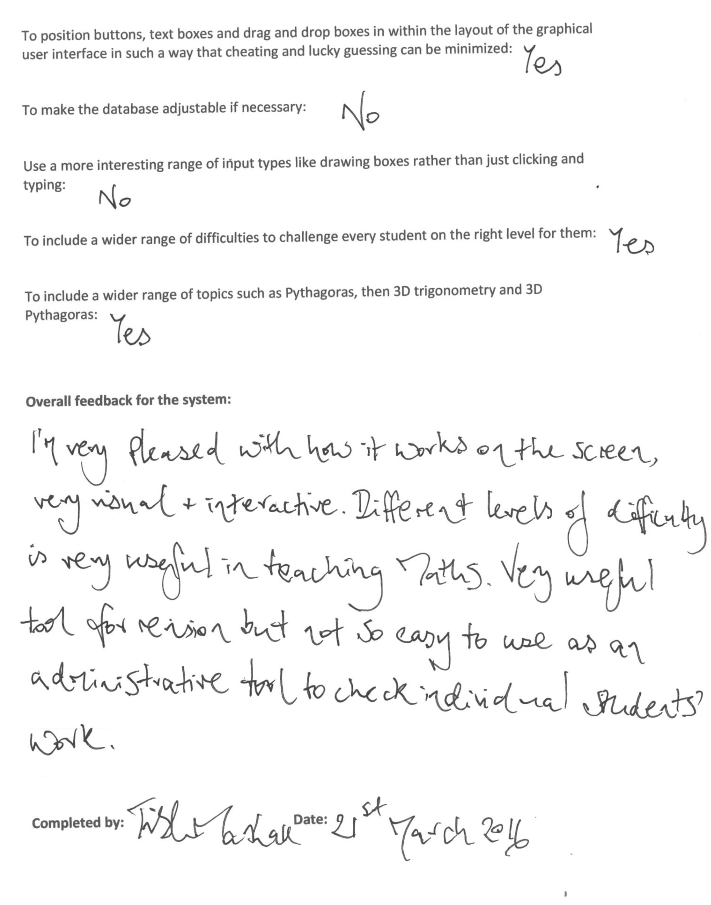
\includegraphics{C:/Users/Jordan/git/COMP4Coursework2/Evaluation/client_feedback_3}
\end{figure}

\subsection{Questionnaires}

This was a brief questionnaire given to the client to give a broad idea of how satisfied they are with the system.

\begin{figure}[H]
	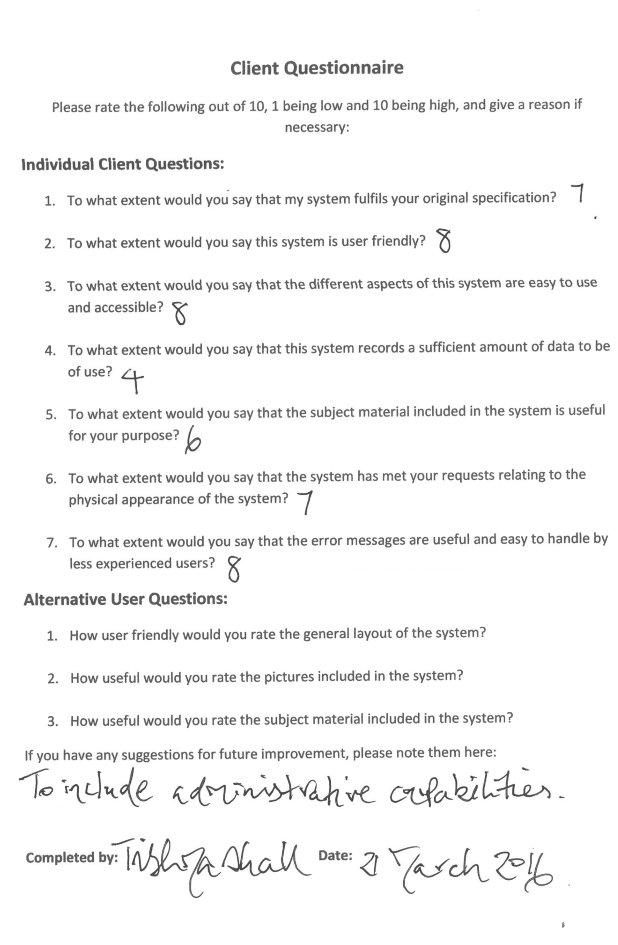
\includegraphics{C:/Users/Jordan/git/COMP4Coursework2/Evaluation/client_questionnaire}
\end{figure}

\subsection{Graphs}

This graph shows the balance of how satisfied the client is with the system:

\begin{figure}[H]
	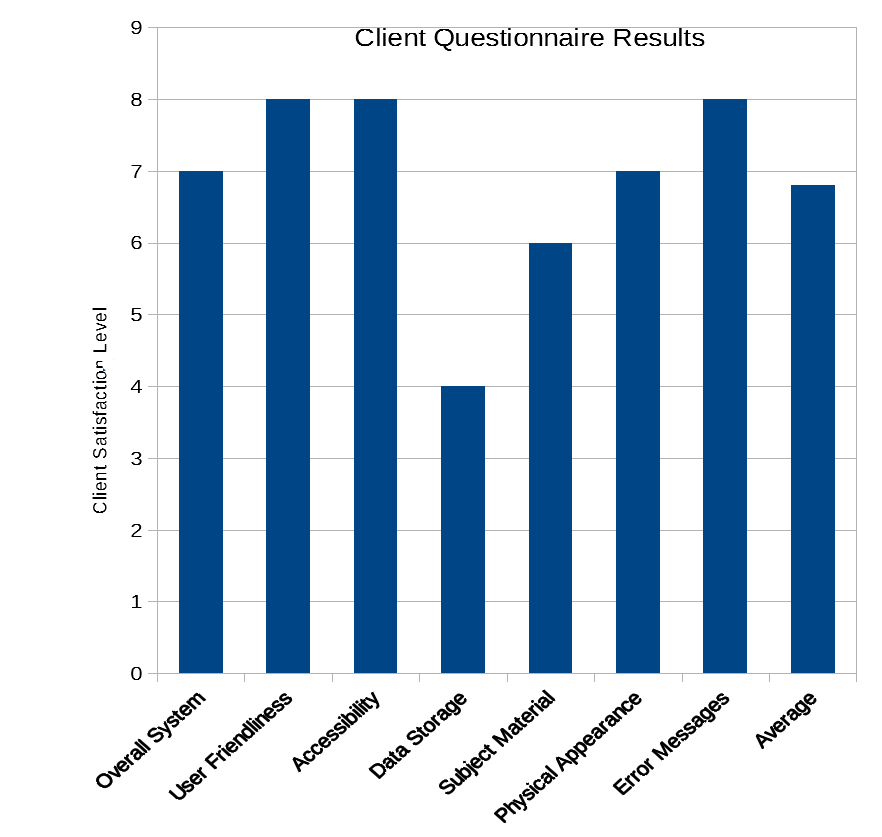
\includegraphics{C:/Users/Jordan/git/COMP4Coursework2/Evaluation/client_graph}
	\caption{According to this graph, the customer was satisfied with 68\% of the system.}
\end{figure}

This graph shows each of the client's 'yes' marks  against the number of 'no' marks related to whether or not each objective was achieved (out of 32 objectives/sub-objectives, some of which were only partially achieved):

\begin{figure}[H]
	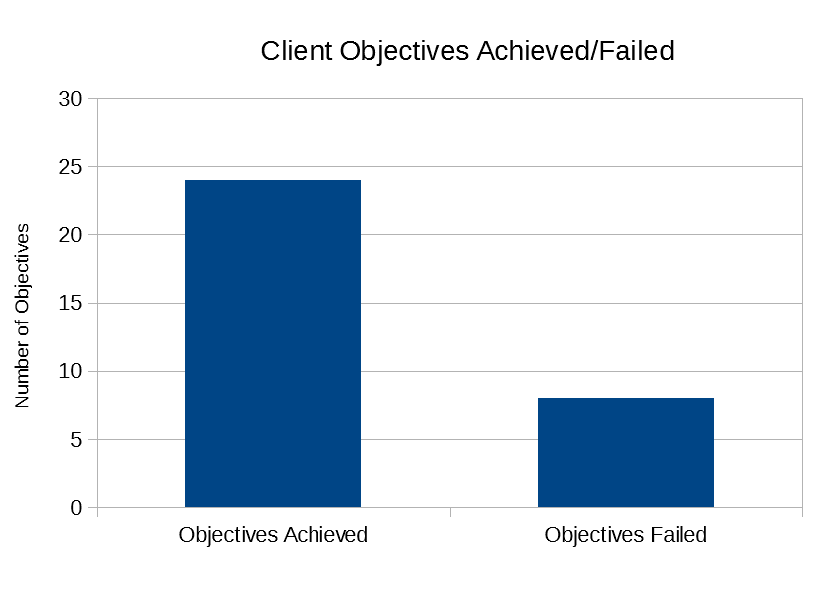
\includegraphics{C:/Users/Jordan/git/COMP4Coursework2/Evaluation/client_graph_2}
	\caption{According to this graph, the customer believed I had achieved 75\% of their specified objectives.}
\end{figure}